\documentclass[review]{elsarticle}

\usepackage{amsmath}
\usepackage{dirtytalk}
\usepackage{subcaption}
\usepackage[usenames]{xcolor}
\usepackage{lineno,hyperref}
\modulolinenumbers[5]

\journal{Composites Part A}

%%%%%%%%%%%%%%%%%%%%%%%
%% Elsevier bibliography styles
%%%%%%%%%%%%%%%%%%%%%%%
%% To change the style, put a % in front of the second line of the current style and
%% remove the % from the second line of the style you would like to use.
%%%%%%%%%%%%%%%%%%%%%%%

%% Numbered
%\bibliographystyle{model1-num-names}

%% Numbered without titles
%\bibliographystyle{model1a-num-names}

%% Harvard
%\bibliographystyle{model2-names.bst}\biboptions{authoryear}

%% Vancouver numbered
%\usepackage{numcompress}\bibliographystyle{model3-num-names}

%% Vancouver name/year
%\usepackage{numcompress}\bibliographystyle{model4-names}\biboptions{authoryear}

%% APA style
%\bibliographystyle{model5-names}\biboptions{authoryear}

%% AMA style
%\usepackage{numcompress}\bibliographystyle{model6-num-names}

%% `Elsevier LaTeX' style
\bibliographystyle{elsarticle-num}
%%%%%%%%%%%%%%%%%%%%%%%

\begin{document}

\begin{frontmatter}

\title{Energy release rate of the fiber/matrix interface crack in cross-ply $\left[0_{k\cdot2n}^{\circ},90_{n}^{\circ}\right]_{S}$ laminates under transverse loading: debond/bi-material interface interaction}
%\tnotetext[mytitlenote]{Fully documented templates are available in the elsarticle package on \href{http://www.ctan.org/tex-archive/macros/latex/contrib/elsarticle}{CTAN}.}

%% Group authors per affiliation:
%\author{Luca Di Stasio\fnref{myfootnote}}
%\address{Radarweg 29, Amsterdam}
%\fntext[myfootnote]{Since 1880.}

%% or include affiliations in footnotes:
\author[nancy,lulea]{Luca Di Stasio}
\author[lulea]{Janis Varna}
\author[nancy]{Zoubir Ayadi}
%\ead[url]{www.elsevier.com}

%\author[mysecondaryaddress]{Global Customer Service\corref{mycorrespondingauthor}}
%\cortext[mycorrespondingauthor]{Corresponding author}
%\ead{support@elsevier.com}

\address[nancy]{Universit\'e de Lorraine, EEIGM, IJL, 6 Rue Bastien Lepage, F-54010 Nancy, France}
\address[lulea]{Lule\aa\ University of Technology, University Campus, SE-97187 Lule\aa, Sweden}

\begin{abstract}
\noindent
%\textcolor{purple}{{\em Priority}: 1}\\
%\textcolor{purple}{{\em Target journal(s)}: Composites Part B: Engineering, Composites Part A: Applied Science and Manufacturing, Composite Structures, Journal of Composite Materials, Composite Communications}\\
The effects of crack shielding, fiber content and ratio of $0^{\circ}$ to $90^{\circ}$ ply thickness on fiber/matrix debond growth in thin cross-ply laminates are investigated with Representative Volume Elements (RVEs) of different ordered microstructures. Debond growth is characterized by the estimation of the Energy Release Rates (ERRs) using the Virtual Crack Closure Technique (VCCT) and the J-integral. It is found that 
\end{abstract}

\begin{keyword}
Polymer-matrix Composites (PMCs)\sep Thin-ply\sep Transverse Failure \sep Debonding \sep Finite Element Analysis (FEA)
\end{keyword}


\end{frontmatter}

\linenumbers

%%%%%%%%%%%%%%%%%%%%%%%%%%%%%%%%%%%%%%%%%%%%%%%%%%%%%%%%%%%%%%%%%%%
% 1. INTRODUCTION
%%%%%%%%%%%%%%%%%%%%%%%%%%%%%%%%%%%%%%%%%%%%%%%%%%%%%%%%%%%%%%%%%%%

\section{Introduction}

Since the development of the \emph{spred tow} technology or \say{FUKUI method}~\cite{Kawabe2008,Kawabe2008en}, significant efforts have been directed toward the characterization of \emph{thin-ply} laminates~\cite{Sasayama2003,Yamaguchi2005,Tsai2005,Sihn2007,Yokozeki2008,Yokozeki2010,Saito2012,Arteiro2013,Arteiro2014,Amacher2014,Guillamet2014,Huang2018,Cugnoni2018} and their application to mission-critical structures in the aerospace sector~\cite{Moon2011,Kim2017,Kopp2017,McCarville2018}.\\
At the lamina level, the use of \emph{thin-plies} leads to more regular and homogeneous microstructures but no significant imporvement in static properties except for an apparent improvement in compressive strength~\cite{Amacher2014}. Improvements in fatigue life have been observed, although contrasting results can be found in the literature~\cite{Yamaguchi2005,Tsai2005,Sihn2007}. The beneficial effect of the use of \emph{thin-plies} with respect to damage propagation has been instead commonly observed by different researchers under static~\cite{Sasayama2003,Sihn2007,Yokozeki2008,Yokozeki2010,Saito2012,Arteiro2013,Arteiro2014,Amacher2014}, fatigue~\cite{Yamaguchi2005,Sihn2007,Yokozeki2008,Yokozeki2010,Amacher2014} and impact loadings~\cite{Sihn2007,Yokozeki2008,Yokozeki2010,Amacher2014}. It seems apparent that \emph{thin-ply} laminates possess an increased ability to delay, and in some cases even suppress, the onset and propagation of transverse cracks (or matrix or micro-cracks).\\
The first appearance of transverse cracking phenomena is known to be characterized by the appearance of fiber/matrix interface cracks (also referred to as debonds), which grow along the fiber's arc direction, then kink out of the interface and coalesce forming a transverse crack~\cite{Bailey1981}. Different approaches have been applied to model the initiation and growth of debonds. The Cohesive Zone Model (CZM) has been used to mimic the propagation of debonds along fiber interfaces; coupled with a failure criterion for the matrix, it has provided simulations of the growth of transverse cracks starting from a virgin material~\cite{Kushch2011,Canal2012,Bouhala2013,Herraez2015}. The main advantages of this approach are the possibility to observe the development of a simulated crack path and to record a load-displacement curve to compare with experimental measurement. However, various observations cast a doubt about the applicability of the CZM: the bi- (for 2D models) and tri- (in 3D) axiality of the matrix stress state in the inter-fiber region that is linked with a cavitation-like failure of the polymer~\cite{Asp1995}; the locality and mode dependency of the interface failure~\cite{Mantic2009}; the problematic use at the microscopic level of properties measured in UD specimens at the laminate level~\cite{Canal2012}. A second approach that obviates these drawbacks is the application of Linear Elastic Fracture Mechanics (LEFM) arguments to the study of debond growth. The analysis focuses on the evaluation of Mode I and Mode II Energy Release Rate (ERR) at the crack tip by means of the Virtual Crack Closure Technique (VCCT)~\cite{Krueger2004} or the J-Integral method~\cite{Rice1968}. The stress and strain field, required for the ERR computation, can be solved by application of different methodologies such as analytical solutions~\cite{Toya1974}, the Boundary Element Method (BEM)~\cite{Paris1996} or the Finite Element Method (FEM)~\cite{Zhuang2018}. Different works have followed this approach and studied models of one or two fibers in an effectively infinite matrix~\cite{Correa2011,Correa2013,Correa2014,Sandino2016,Sandino2018} and of an hexagonal cluster of fibers in an effectively infinite homogenized UD composite~\cite{Varna2017,Zhuang2018}. The problem of debond growth along the fiber-matrix interface in a cross-ply laminate has been only addressed very recently in~\cite{Velasco2018,Paris2018}, where the author embed a single partially debonded fiber in an effectively infinite homogenized $90^{\circ}$ ply bounded by homogenized $0^{\circ}$ layers. Thus, the effect of debond-debond interaction and of the relative proximity of a bi-material interface on the debond's ERR in cross-ply laminates is yet to be addressed. The present work is devoted to this problem. Models of Repeating Unit Cells (RUCs) are developed to represent laminates with different degrees of damage (here only in the form of debonds). The number of fully bonded fibers across the thickness of the $90^{\circ}$ ply is varied in order to investigate the effect of the proximity of the bi-material interface. The thickness of the bounding $0^{\circ}$ layers is also analyzed as a parameter of the study. The stress and strain fields are solved with the Finite Element Method in Abaqus~\cite{abq12} and the crack characterized by its Mode I and Mode II ERR, calculated with the VCCT and the J-integral method.

%%%%%%%%%%%%%%%%%%%%%%%%%%%%%%%%%%%%%%%%%%%%%%%%%%%%%%%%%%%%%%%%%%%
% 2. RVE MODELS AND FE DISCRETIZATION
%%%%%%%%%%%%%%%%%%%%%%%%%%%%%%%%%%%%%%%%%%%%%%%%%%%%%%%%%%%%%%%%%%%

\section{RVE models \& FE discretization}

% 2.1 Introduction and nomenclature

\subsection{Introduction \& Nomenclature}\label{subsec:names}

In the present work, we investigate debond development in cross-ply $\left[0_{k\cdot2n}^{\circ},90_{n}^{\circ}\right]_{S}$ laminates under in-plane transverse tension. The interaction between debonds in the presence of a stiff bi-material interface is studied with the use of different RUCs (see Figures~\ref{fig:laminateModelsA} and~\ref{fig:laminateModelsB} in Sec.~\ref{subsec:rve}), in which only the central fiber presents damage in the form of a debond. Repetition of the composite RUC can occur only along the in-plane transverse direction only, thus representing a cross-ply laminate with a thin or even ultra-thin $90^{\circ}$ ply in the middle.\\
The thickness of the $90^{\circ}$ ply depends on the number of fibers present across the thickness (the vertical or $z$ direction in Figures~\ref{fig:laminateModelsA} and~\ref{fig:laminateModelsB}) and the value of the fiber volume fraction $V_{f}$. On the other hand, the thickness of the $0^{\circ}$ layers can be assigned freely as a multiple of the $90^{\circ}$ ply thickness, i.e. $t_{0^{\circ}}=i\cdot t_{90^{\circ}}$ where $i$ is an arbitrary integer. The thickness ratio $i$ could in theory be assumed to be a real positive number; however, it seems more reasonable to consider it only as a positive integer based on practical considerations on the actual manufacturing  of laminates (stacking of a discrete number of pre-impregnated layers). Thus, the thickness ratio $i$ represents one additional parameter for the investigation. In the RUCs proposed, we consider the $90^{\circ}$ ply with debonds as a series of stacked damaged and undamaged fiber rows, each row with only one fiber in the thickness direction. All the RUCs present regular microstructures with fibers placed according to a square-packing configuration and consequently they are Representative Volume Elements (RVE) of cross-ply laminates with a certain distribution of debonds in the middle $90^{\circ}$ layer. In the following, let us consider in-plane coordinates $x$ and $y$, where $x$ is in the transverse direction of the cross-ply laminate under consideration. In the presence of a load in the $x$-direction, the strain in the $y$-direction is small, due to the very small minor Poisson's ratio of the laminate. Furthermore, debonds are considered to be significantly longer in the fiber direction than in the arc direction~\cite{Zhang1997}. Therefore we use 2D models under the assumption of plane strain, defined in the $x-z$ section of the composite. The study presented in this paper thus applies to long debonds and its focus ia on understanding the mechanisms of growth along their arc direction. The laminates are assumed to be subject to transverse tensile strain, which is applied in the form of a constant displacement in the $x$-direction along both vertical boundaries of the RUC as shown in  Figure~\ref{fig:modelschem}.\\
In summary, the models are differentiated by: first, the spacing between debonds along the horizontal direction in the $90^{\circ}$ layer, which corresponds to the number $n$ of fibers in the RUC's horizontal direction; second, the thickness of the middle $90^{\circ}$ ply measured in terms of the number $k$ of fiber rows; third, the factor $i$ which provides the thickness of the $0^{\circ}$ layers as an integer multiple of the $90^{\circ}$ ply thickness.  It thus seems natural to introduce the common notation $n\times k-i\cdot t_{90^{\circ}}$. A final additional model is considered to study the effect of equivalent boundary conditions~\ref{subsec:eqBC}. This final model is constituted by only one partially debonded fiber. The application of coupling of horizontal displacements in the form of a constant applied displacement along the right and left sides allows for repetition along the horizontal direction. The presence of coupling of vertical displacements and a linear distribution of horizontal displacements on the bottom and top surfaces models the presence of the stiff bi-material interface between the $90^{\circ}$ and the $0^{\circ}$ layers. This model is refered to as $1\times 1-H+V$ given that: it has respectively 1 fiber in the horizontal and in the vertical direction; on the top and bottom surfaces, both horizontal (H) and vertical (V) displacements are assigned.  

% 2.2 Models of Representative Volume Element (RVE)

\subsection{Models of Representative Volume Element (RVE)}\label{subsec:rve}

The first family of models is represented in Figure~\ref{fig:laminateModelsA}. It represents a set of $\left[0_{k\cdot2n}^{\circ},90_{n}^{\circ}\right]_{S}$ cross-ply laminates with an ultra-thin $90^{\circ}$ layer, constituted by a single row of fibers across the thickness. Debonds appear at regular intervals measured in terms of number $n$ of fully bonded fibers present between them, which in turn correspond to the number of fibers along the horizontal direction of the RUC as highlighted in Fig.~\ref{fig:laminateModelsA}. They are thus the $n\times1-i\cdot t_{90^{\circ}}$ models, where $i=1,10$ and $n$ is an integer $\geq1$ ($n=1$ corresponds to the case of a debond appearing on all the fibers in the central $90^{\circ}$ layer). These models are quite extreme, but allow to focus on the interaction between debonds and the inter-ply bi-material interface. Furthermore, the \emph{spread tow} technology is today capable of producing cross-ply laminates with the central $90^{\circ}$ layer thickness only $4-5$ times the fiber diameter, as shown for example in~\cite{Saito2012}, which give practical relevance even to such extreme models.  

\begin{figure}[!h]
\centering
  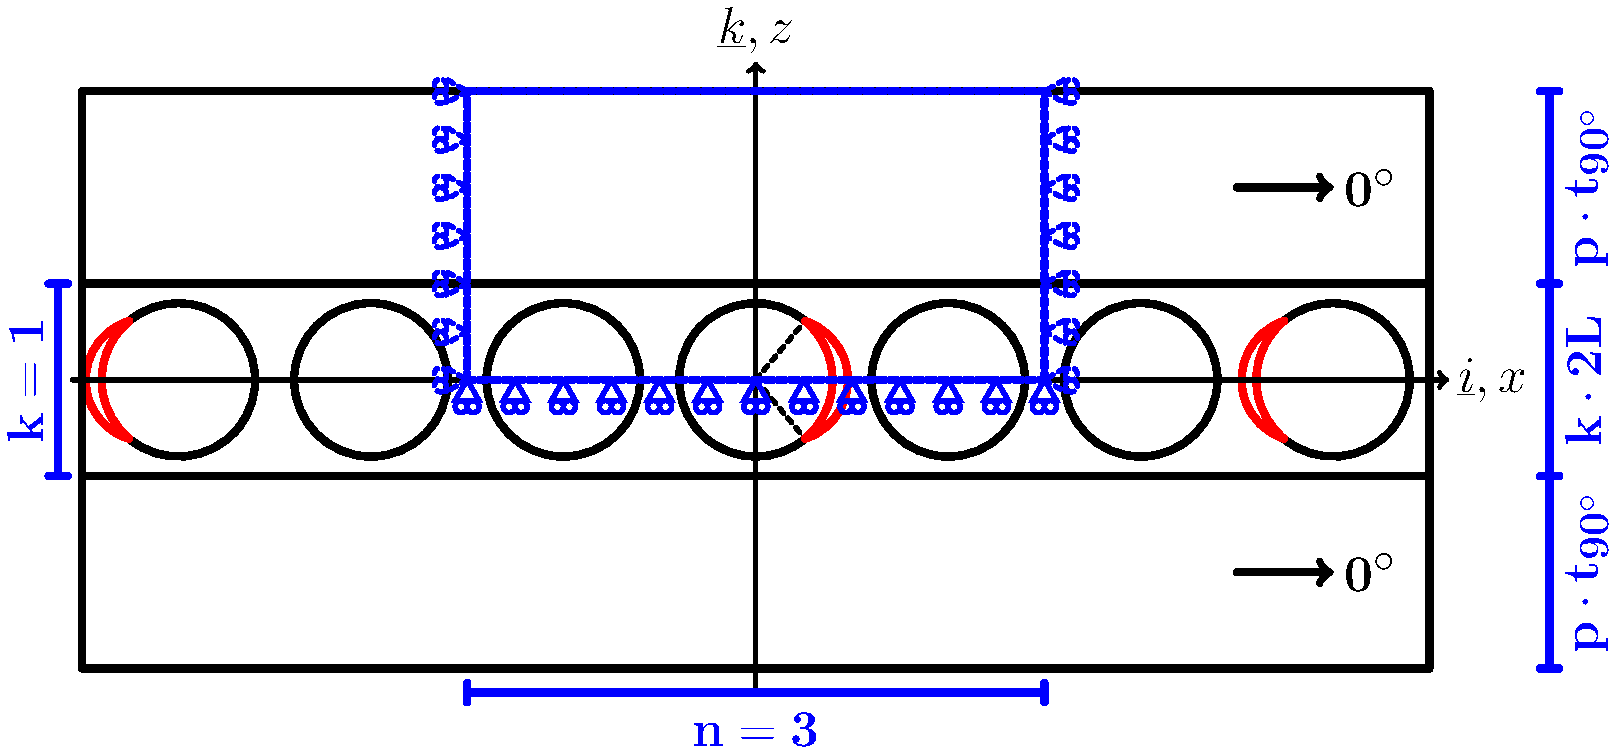
\includegraphics[width=\textwidth]{thinPly.pdf}
\caption{Models of $\left[0_{k\cdot2n}^{\circ},90_{n}^{\circ}\right]_{S}$ cross-ply laminates with an ultra-thin $90^{\circ}$ layer, where the $90^{\circ}$ ply is made up by a single ``row'' of fibers. Debonds are repeating at different distances, measured in terms of the number $n$ of fully bonded fibers appearing between two consecutive debonds.}\label{fig:laminateModelsA}
\end{figure}

The second set of models considers instead cross-ply laminates with a central $90^{\circ}$ ply of variable thickness, measured in terms of number $k$ of fiber rows appearing in the vertical direction in Figure~\ref{fig:laminateModelsB}. Once again, debonds appear at regular intervals measured in terms of number $n$ of fully bonded fibers present between them, which in turn correspond to the number of fibers along the horizontal direction of the RUC as highlighted in Fig.~\ref{fig:laminateModelsB}. These models are thus the $n\times k-i\cdot t_{90^{\circ}}$ models, where $i=1,10$, $k>1$ and $n$ is an integer $\geq1$ ($n=1$ corresponds to the case of a debond appearing on all the fibers of the central fiber row in the $90^{\circ}$ layer).

\begin{figure}[!h]
\centering
        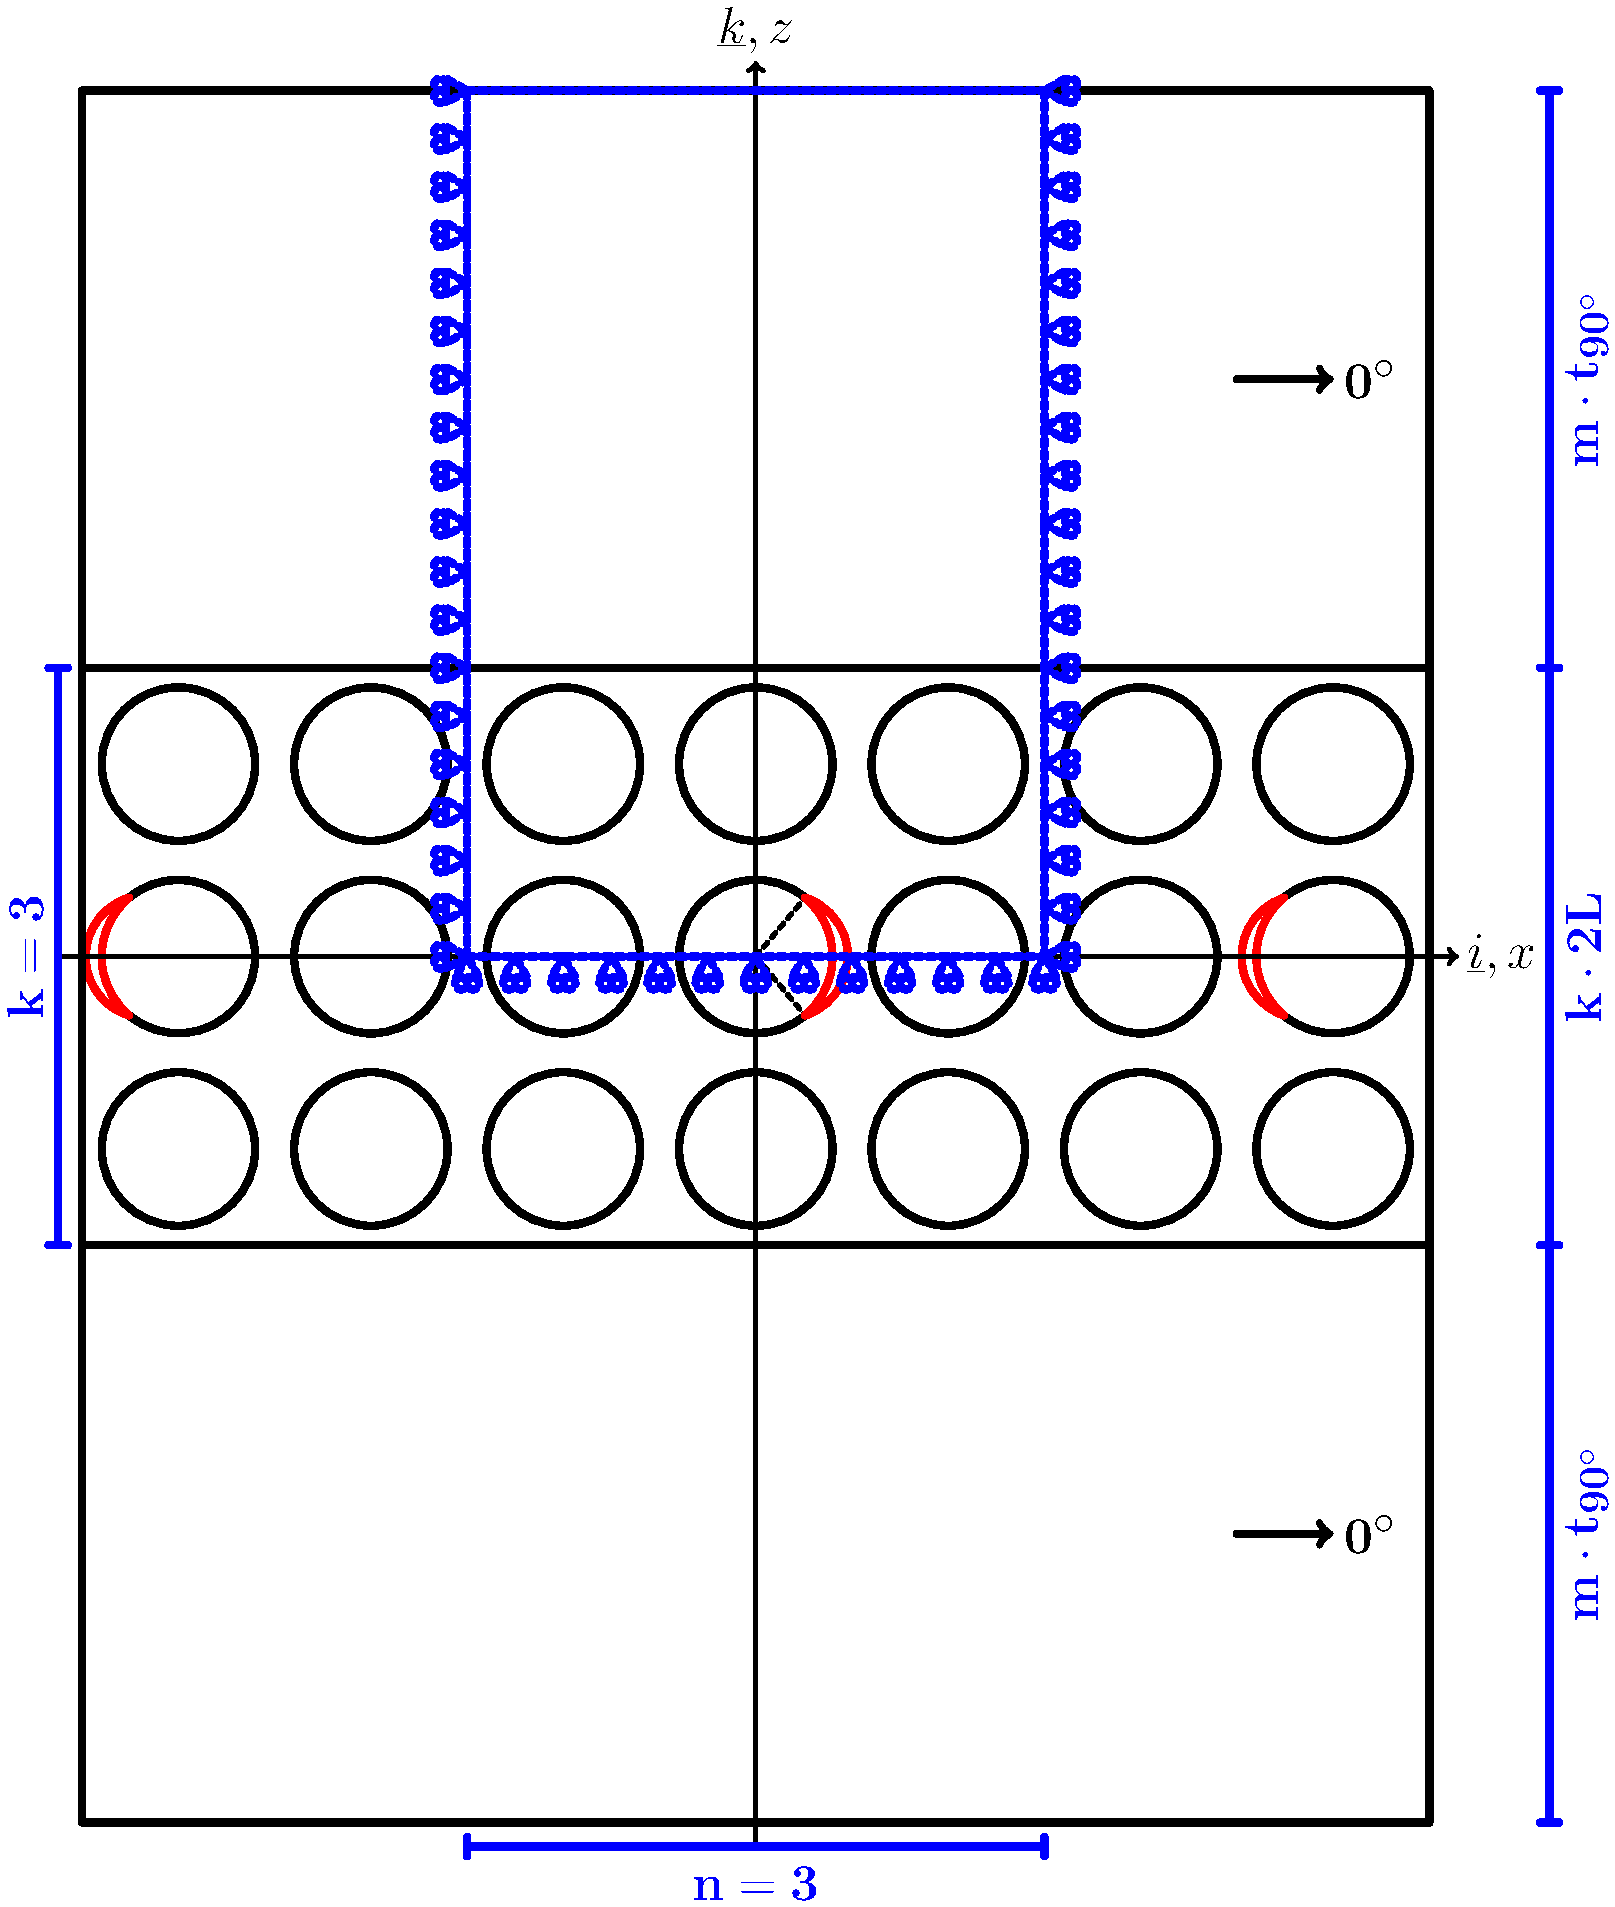
\includegraphics[width=\textwidth]{ThickPly.pdf}
   %    \caption{Mutiple rows of fibers with a debond appearing every $n$ fibers within the central row: model $n\times k-free$ ($n=3$ and $k=3$ in the figure).}\label{subfig:thickply}
\caption{Models of $\left[0_{k\cdot2n}^{\circ},90_{n}^{\circ}\right]_{S}$ cross-ply laminates with a $90^{\circ}$ layer of variable thickness, determined by the number $k$ of ``rows'' of fibers along the vertical direction.  Debonds are repeating at different distances along the horizontal direction, measured in terms of the number $n$ of fully bonded fibers appearing between two consecutive debonds.}\label{fig:laminateModelsB}
\end{figure}

By increasing the number $n$ of fibers in the horizontal direction in the RUC, decreasing levels of damage (debonds spaced further apart) are considered to be present in the laminate. By increasing the number $k$ of fiber rows, the thickness of the $90^{\circ}$ layer is increased and the effect of the relative proximity of the inter-ply bi-material interface can thus be studied. Finally, by increasing the factor $i$, the thickness of the $0^{\circ}$ layers is increased for a given thickness of the $90^{\circ}$, which allows the investigation of the size effect or \emph{in-situ} effect for the fiber-matrix interface crack.

% 2.3 Finite Element (FE) discretization

\subsection{Finite Element (FE) discretization}

\begin{figure}[!h]
\centering
        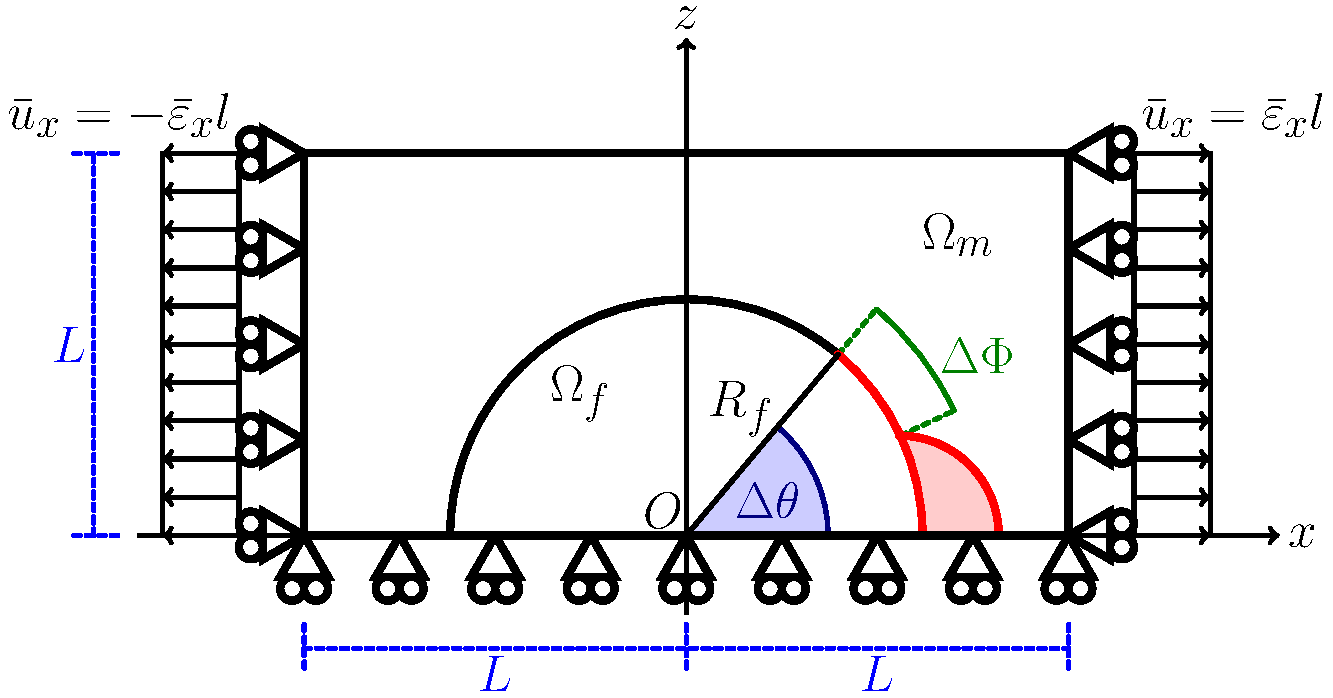
\includegraphics[width=\textwidth]{RUC.pdf}
\caption{Schematic of the model with its main parameters.}\label{fig:modelschem}
\end{figure}

%%%%%%%%%%%%%%%%%%%%%%%%%%%%%%%%%%%%%%%%%%%%%%%%%%%%%%%%%%%%%%%%%%%
% 3. RESULTS AND DISCUSSION
%%%%%%%%%%%%%%%%%%%%%%%%%%%%%%%%%%%%%%%%%%%%%%%%%%%%%%%%%%%%%%%%%%%

\section{Results \& Discussion}

\subsection{Interaction between debonds in a $90^{\circ}$ ply with a single layer of fibers inside a $\left[0^{\circ}_{n}, 90^{\circ}\right]_{S}$ laminate}


\subsection{Interaction between layers of fully bonded fibers and a centrally located line of debonded fibers in a $90^{\circ}$ ply inside a $\left[0^{\circ}_{n}, 90^{\circ}\right]_{S}$ laminate}



\subsection{Interaction of debonds within a $90^{\circ}$ ply with multiple layers of fibers inside a $\left[0^{\circ}_{n}, 90^{\circ}\right]_{S}$ laminate}

\subsection{Comparison with the single fiber model with equivalent boundary conditions}\label{subsec:eqBC}

%%%%%%%%%%%%%%%%%%%%%%%%%%%%%%%%%%%%%%%%%%%%%%%%%%%%%%%%%%%%%%%%%%%
% 4. CONCLUSIONS AND OUTLOOK
%%%%%%%%%%%%%%%%%%%%%%%%%%%%%%%%%%%%%%%%%%%%%%%%%%%%%%%%%%%%%%%%%%%

\section{Conclusions \& Outlook}

%%%%%%%%%%%%%%%%%%%%%%%%%%%%%%%%%%%%%%%%%%%%%%%%%%%%%%%%%%%%%%%%%%%
% ACKNOWLEDGEMENTS
%%%%%%%%%%%%%%%%%%%%%%%%%%%%%%%%%%%%%%%%%%%%%%%%%%%%%%%%%%%%%%%%%%%

\section*{Acknowledgements}

Luca Di Stasio gratefully acknowledges the support of the European School of Materials (EUSMAT) through the DocMASE Doctoral Programme and the European Commission through the Erasmus Mundus Programme.

%%%%%%%%%%%%%%%%%%%%%%%%%%%%%%%%%%%%%%%%%%%%%%%%%%%%%%%%%%%%%%%%%%%
% REFERENCES
%%%%%%%%%%%%%%%%%%%%%%%%%%%%%%%%%%%%%%%%%%%%%%%%%%%%%%%%%%%%%%%%%%%

\bibliography{refs}

\end{document}
